\textcolor{red}{Rectifier le tir des maillages simples / lisses}
\textcolor{red}{Virer les "maillages basiques"}

\begin{figure}[h!]
	\adjustbox{center}{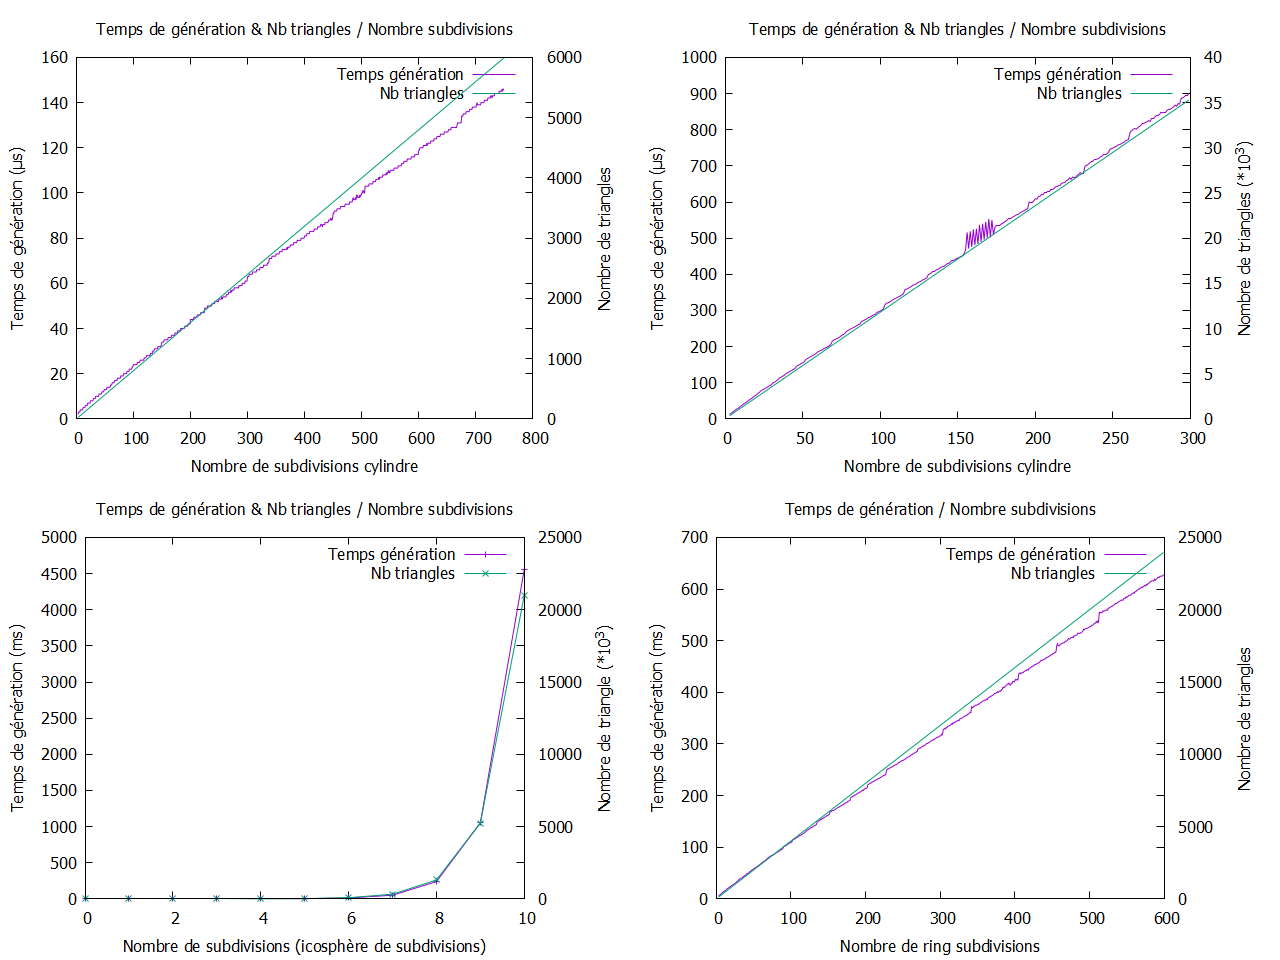
\includegraphics[width=1.2\textwidth]{Captures/allBenchmarksTriangles.png}}

	\caption{Temps de génération pour les maillages simples implémentés en fonction du nombre de subdivisions}
\end{figure}
\FloatBarrier

Toutes les primitives à l'exception de l'icopshère évoluent en temps linéaire quand leur nombre de subdivisions 
augmente et c'est le comportement auquel on pourrait s'attendre. L'icosphère évolue en $4^n$ avec $n$ le nombre 
de subdivisions (le graphique de l'icosphère a son axe des ordonnées en échelle logarithmique base 4). C'est 
également ce à quoi on s'attend puisque la subdivision dyadique multiplie par 4 le nombre de triangles à chaque subdivision.

Les courbes montrent des "accidents", elles ne sont pas totalement "lisses" et cela est dû à différents aspects techniques tels
que la taille des caches du CPU, les réallocations des \textit{std::vector} lors de \textit{push\_back()}, ...
